




\title[概率论]{第十一讲:多维概率分布}
%\author[张鑫 {\rm Email: x.zhang.seu@foxmail.com} ]{\large 张 鑫}
\institute[东南大学数学学院]{\large \textrm{Email: xzhangseu@seu.edu.cn} \\ \quad  \\
	\large 东南大学 \quad 数学学院 \\
	\vspace{0.3cm}
	% \trc{公共邮箱: \textrm{zy.prob@qq.com}\\
		%    \hspace{-1.7cm}  密 \qquad 码: \textrm{seu!prob}}
}
\date{\rm \today}

{ \setbeamertemplate{footline}{}
  \begin{frame}
    \titlepage
  \end{frame}
}

% \begin{frame}[plain]
%   \frametitle{目录}
%   \setcounter{tocdepth}{2}
%   \tableofcontents
% \end{frame}
\addtocounter{framenumber}{-3}  % 目录页不计算页码
%\section{随机变量}
\subsection{多维概率分布}
\begin{frame}
  \frametitle{$n$ 维随机向量的定义}
  \begin{defi}[$n$ 维随机向量或随机变量] 如果 $X_1,\cdots, X_n$ 是定义在同一个概率空间 $(\Omega,\mathcal{F},P)$ 上的 $n$ 个随机变量,即
    \begin{eqnarray*}
      \{\omega:X_i (\omega)\in B_i\}\in \mathcal{F}, \quad \mbox{任意的} B_i\in \mathcal{B},
    \end{eqnarray*}
    则称 $X (\omega):=(X_1 (\omega),\cdots,X_n (\omega))$ 为概率空间 $(\Omega,\mathcal{F},P)$ 上的 $n$ 维随机向量或 $n$ 维随机变量.
  \end{defi}

\vspace{0.2cm}
\begin{rmk}
	\begin{itemize}[<+-|alert@+>]
		\item 如果 $\left (X_1,\cdots ,X_n \right) $ 是一个 $n$ 维随机向量,则对任何不超过 $n$ 的正整数 $k$ 和 $1\leqslant j_1<\cdots <j_k\leqslant n$, $\left ( X_{j_1},\cdots ,X_{j_k} \right) $
		都是一个 $k$ 维随机向量;
		\item 特别地,当 $k=1$ 时就是随机变量.
	\end{itemize}

\end{rmk}

\end{frame}
\begin{frame}{$n$ 维随机向量的定义}


	\begin{thm}
		$X (\omega)=(X_1 (\omega),\cdots,X_n (\omega))$ 是定义在某个概率空间 $(\Omega,\mathcal{F},P)$ 上的 $n$ 维随机向量当且仅当对任意的 $(x_1,\cdots, x_n)\in \mathbb{R}^ n$ 均有
		\[\{\omega: X_1(\omega)\leq x_1,\cdots, X_n(\omega)\leq x_n\}=\{X_1\leq x_1,\cdots, X_n\leq x_n\}\in\mathcal{F},\]
		或等价的有对任意的 $B\in\mathcal{B}(\mathbb{R}^ n)$
		\[\{\omega: X(\omega)\in B\}=\{\omega: (X_1(\omega),\cdots,X_n(\omega))\in B\}\in\mathcal{F}.\]
	\end{thm}


\end{frame}

\subsection{多维分布}
\begin{frame}{多维分布及联合分布函数}
		\begin{defi}[多维分布]
		设 $X=\left (X_1,\cdots ,X_n \right) $ 是定义在某个概率空间 $\left ( \varOmega ,\mathcal{F},P   \right) $ 上的 $n$ 维随机向量,则对任意的 $B\in\mathcal{B}(\mathbb{R}^n)$, 称
		$$
		\mathbf{F}(B):=P(X\in B)=P((X_1,\cdots, X_n)\in B)
		$$ 为 $n$ 维随机向量 $X=\left (X_1,\cdots ,X_n \right)$ 的分布. % 为其分布函数,也称为随机变量 $ X_1,\cdots ,X_n$ 的联合分布函数.
	\end{defi}

\pause

	\begin{defi}[分布函数或联合分布函数]
		设 $X=\left (X_1,\cdots ,X_n \right) $ 是定义在某个概率空间 $\left ( \varOmega ,\mathcal{F},P \right) $ 上的 $n$ 维随机向量,称
		$$
		F\left( x_1,\cdots ,x_n \right) =P\left( X_1\leqslant x_1,\cdots ,X_n\leqslant x_n \right) ,\quad \forall \left( x_1,\cdots ,x_n \right) \in \mathbb{R}^n
		$$ 为随机向量 $X$ 的分布函数,也称为随机变量 $ X_1,\cdots,X_n$ 的联合分布函数.
	\end{defi}
\pause
\begin{rmk}
\begin{itemize}[<+-|alert@+>]
	\item $n$ 维随机向量的分布函数 $F (x_1,\cdots,x_n)$ 是定义在 $\mathbb{R}^n$ 上的 $n$ 元函数;
	\item 称一个 $n$ 元函数 $F (x_1,\cdots,x_n)$ 为 $n$ 维分布函数,如果存在某个随机向量以它作为分布函数.
\end{itemize}
\end{rmk}

\end{frame}

\begin{frame}{$n$ 维随机向量分布函数的性质}
	\vspace{-0.15cm}
	\begin{thm}
	 	$n$ 维随机向量 $X=\left (X_1,\cdots ,X_n \right)$ 的分布函数 $F\left ( x_1,\cdots ,x_n \right)$ 具有下述性质:
		\begin{enumerate}[<+-|alert@+>]
			\item $F\left (x_1,\cdots ,x_n \right)$ 对每个变元非降;
			\item $F\left (x_1,\cdots ,x_n \right)$ 对每个变元右连续;
			\item 对任意的 $1\leq j\leq n$, $$
			\begin{aligned}
				&\lim_{x_j\rightarrow -\infty} F\left( x_1,\cdots, x_j,\cdots,x_n \right) =0,\\
				&\lim_{x_1\rightarrow \infty ,\cdots ,x_n\rightarrow \infty} F\left( x_1,\cdots ,x_n \right) =1\\
			\end{aligned}
			$$
			\item $F\left (x_1,\cdots ,x_n\right)$ 具有增量非负性:对任意的 $1\leq j\leq n$ 及 $a_j\leqslant b_j$ 均有 %,j=1,\cdots ,n,$ 都有
			$$
			\Delta_{\left(a_{1}, \cdots, a_{n}\right)}^{\left(b_{1}, \cdots, b_{n}\right)} F=\sum_{\boldsymbol{x}=(x_1,\cdots, x_n)\in\mathcal{O}} \operatorname{sgn}(\boldsymbol{x}) F(\boldsymbol{x}) \geqslant 0,
			$$
			其中 \vspace{-0.5cm}
			\begin{align*}
				\mathcal{O}&:=\{(x_1,\cdots,x_n): x_j=a_j\mbox{或} b_j, 1\leq j\leq n\},\\
				\operatorname{sgn}(\boldsymbol{x})&=\left\{
				\begin{array}{ll}
					1,& |\{j:x_j=a_j\}|\mbox{为偶数},\\
					-1, &|\{j:x_j=a_j\}|\mbox{为奇数}.
					\end{array}\right.
			\end{align*}
%			其中共有 $2^n$ 个加项,$\boldsymbol{x}=\left ( x_1,\cdots ,x_n \right) $,有 $x_j=a_j$ 或 $b_j,j=1,\cdots ,n,$,并且当 $\sharp \left\{ j\mid x_j=a_j \right\} $ 为偶数时,${sgn}(\boldsymbol{x})$ 为 $+$ 号,当 $\sharp \left\{ j\mid x_j=a_j \right\} $ 为奇数时,${sgn}(\boldsymbol{x})$ 为 $-$ 号,其中 $\sharp \left\{ \cdot \right\} $ 表示集合 $\left\{ \cdot \right\} $ 中的元素个数.
		\end{enumerate}
	\end{thm}

\end{frame}
\begin{frame}{$n$ 维随机向量分布函数的性质}

特别的,当 $n=2$ 或 3 时,$\Delta_{\left (a_{1}, \cdots, a_{n}\right)}^{\left (b_{1}, \cdots, b_{n}\right)} F$ 有以下具体形式:
\begin{align*}
	\Delta_{\left(a_{1}, a_{2}\right)}^{\left(b_{1}, b_{2}\right)} F&= F\left(b_{1}, b_{2}\right)-F\left(a_{1}, b_{2}\right)-F\left(b_{1}, a_{2}\right)+F\left(a_{1}, a_{2}\right) \pause \\
	\Delta_{\left(a_{1}, a_{2}, a_{3}\right)}^{\left(b_{1}, b_{2}, b_{3}\right)} F&= F\left(b_{1}, b_{2}, b_{3}\right)-F\left(a_{1}, b_{2}, b_{3}\right)-F\left(b_{1}, a_{2}, b_{3}\right)\\
	&\quad -F\left(b_{1}, b_{2}, a_{3}\right) +F\left(a_{1}, a_{2}, b_{3}\right)+F\left(a_{1}, b_{2}, a_{3}\right)\\
	&\quad +F\left(b_{1}, a_{2}, a_{3}\right)-F\left(a_{1}, a_{2}, a_{3}\right)
\end{align*}





\end{frame}


\begin{frame}
  \frametitle{二维 (联合) 分布函数}
  \begin{defi}
    设 $(X,Y)$ 为 $(\Omega,\mathcal{F},P)$ 上的随机向量,称
    \begin{eqnarray*}
      F(x,y):=P(X\le x, Y\le y)
    \end{eqnarray*}
    为 $(X,Y)$ 的二维 (联合) 分布函数.
  \end{defi}
  % \vspace{-1cm}
  \begin{figure}[h]
    \centering
    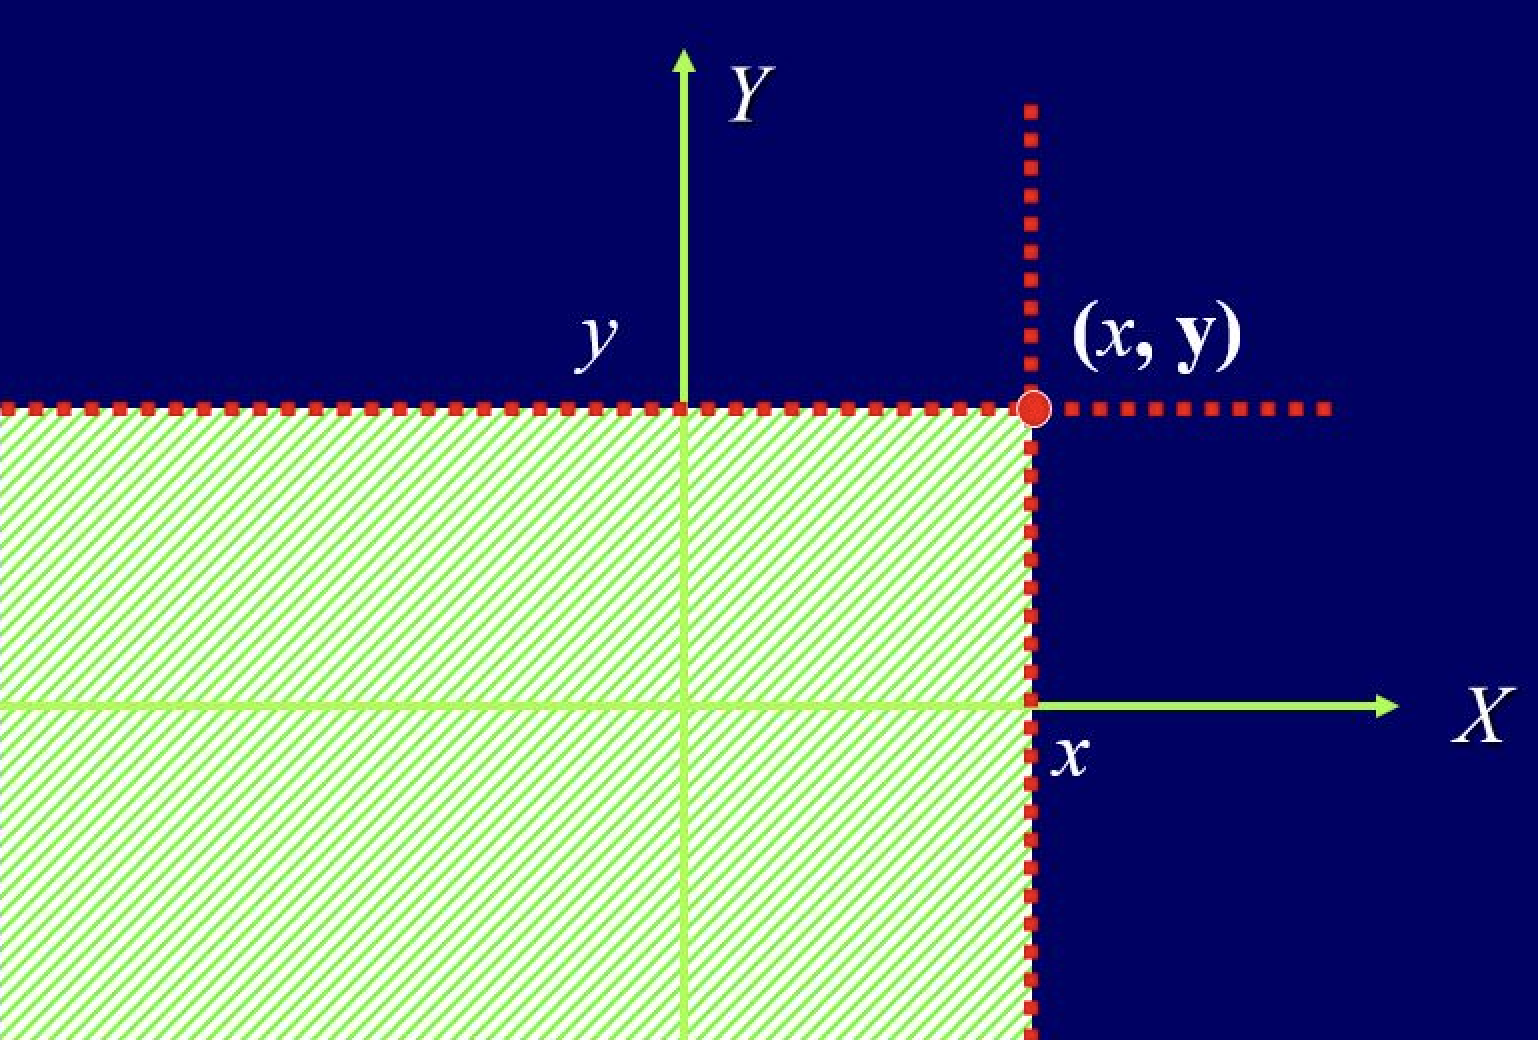
\includegraphics[width=7cm]{fxy.jpg}
    % \caption{高斯}
  \end{figure}

\end{frame}
\begin{frame}
  \frametitle{二维 (联合) 分布函数的性质}
  \begin{thm}
    $F (x,y)$ 具有性质
    \begin{enumerate}[<+-|alert@+>]
    \item $F (x,y)$ 对每个自变量是单调不减的;
    \item $F (x,y)$ 对每个自变量都是右连续的;
    \item{\small $\lim_{x\rightarrow -\infty}F(x,y)=\lim_{y\rightarrow -\infty}F(x,y)=1-\lim_{x\rightarrow +\infty, y\rightarrow +\infty }F(x,y)=0$;}
    \item $F (x,y)$ 在任一矩形 $(a_1,b_1]\times (a_2,b_2]$ 上具有非负增量,即有
      \begin{eqnarray*}
        \Delta F=F(b_1,b_2)-F(a_1,b_2)-F(b_1,a_2)+F(a_1,a_2)\ge 0.
      \end{eqnarray*}

    \end{enumerate}

  \end{thm}
\end{frame}
\begin{frame}
  \frametitle{二维离散型分布}
  \begin{defi}
    若随机向量 $(X,Y)$ 有至多可列对可能值 $(x_i,y_i), i,j=1,2,\cdots,$, 则称随机向量及其联合分布是离散型的,而
    \begin{eqnarray*}
      p_{ij}:=P(X=x_i,Y=y_j), \quad i, j=1,2,\cdots,
    \end{eqnarray*}
    称为 $(X,Y)$ 的联合分布列 (律). 我们常用下表来表示 $(X,Y)$ 的分布列
  \end{defi}
  % \vspace{-1cm}
  \begin{figure}[h]
    \centering
    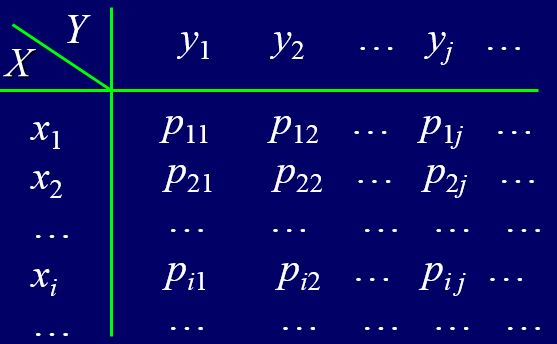
\includegraphics[width=6cm]{pij.jpg}
    % \caption{高斯}
  \end{figure}

\end{frame}
\subsection{二维离散及连续型分布}
\begin{frame}
  \frametitle{二维离散型分布列的基本性质}
  \begin{itemize}[<+-|alert@+>]
  \item 非负性: $p_{ij}\ge 0, i,j=1,2,\cdots $;
  \item 正则性: $\sum_i\sum_jp_{ij}=1$;
  \item 与一维情形类似,对任意的 $B\in \mathcal{B}^2$,
    \begin{eqnarray*}
      P((X,Y)\in B)=\sum_{i, j: (x_i,y_j)\in B}p_{ij}.
    \end{eqnarray*}

  \end{itemize}
\end{frame}
\begin{frame}
  \frametitle{计算联合分布列的方法}
  \begin{itemize}[<+-|alert@+>]
  \item 确定随机变量 $(X, Y)$ 的所有取值数对;
  \item 计算取每个数值对的概率;
  \item 列出表格
  \end{itemize}
  \pause
  \begin{exam}
    从 $1,2,3,4$ 中任取一数记为 $X$, 再从 $1,\cdots,X$ 中任取一数记作 $Y$, 求 $(X,Y)$ 的联合分布列及 $P (X=Y)$.
  \end{exam}
\end{frame}
\begin{frame}
  \frametitle{二维连续型分布}
  \begin{defi}
    若存在二元非负可积函数 $p (x,y)$ 使得 $(X,Y)$ 的二维 (联合) 分布函数
    \begin{eqnarray*}
      F(x,y)=\int_{-\infty}^x\int_{-\infty}^yp(u,v)dudv, \forall (x,y)\in\mathbb{R}^2
    \end{eqnarray*}
    则称 $(X,Y)$ 及其概率分布为连续型的,称 $p (x,y)$ 为其联合分布密度.
  \end{defi}
  \vspace{0.5cm}

  \pause
  易知,联合分布密度具有以下两个基本性质:
  \begin{enumerate}[<+-|alert@+>]
  \item 非负性: $p (x,y)\ge 0$;
  \item 正则性: $\int_{-\infty}^\infty\int_{-\infty}^\infty p (x,y) dxdy=1$.
  \end{enumerate}



\end{frame}
\begin{frame}
  \frametitle{联合分布密度与概率分布之间的关系}

  \begin{itemize}[<+-|alert@+>]
  \item $p(x,y)=\dfrac{\partial^2F(x,y)}{\partial x\partial y}$
  \item 对于连续型随机变量,对任意的 $B\in \mathcal{B}^2$ 有
    \begin{eqnarray*}
      P((X,Y)\in B)=\iint_Bp(x,y)dxdy
    \end{eqnarray*}

  \end{itemize}

\end{frame}
\begin{frame}

  \begin{exam}
    设 $(X,Y)$ 的联合密度函数为
    \begin{eqnarray*}
      p(x,y)=\left\{
      \begin{array}{ll}
        Ae^{-2x-3y},& x>0,y>0\\
        0,&\mbox{其他}
      \end{array}\right.
    \end{eqnarray*}
    试确定常数 $A$, 并求概率 $P (X<2,Y<1)$ 及 $P (2X+3Y<6)$.
  \end{exam}

  \jieda
  \begin{itemize}[<+-|alert@+>]
  \item 由 $\iint p (x,y) dxdy=1$ 可得 $A=6$;
  \item $P(X<2,Y<1)=\pause \int_{-\infty}^2\int_{-\infty}^1p(x,y)dxdy=\pause \int_0^2\int_0^1p(x,y)dxdy=\pause (1-e^{-4})(1-e^{-3})$;
  \end{itemize}

  % \vspace{-1.5cm}
  \begin{figure}[h]
    \centering
    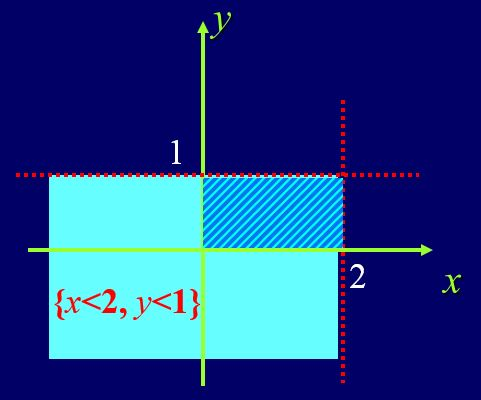
\includegraphics[width=4.8cm]{exam1.jpg}
    % \caption{高斯}
  \end{figure}
\end{frame}
\begin{frame}
  \vspace{0.8cm}
  注意到如果我们令 $D:=\{(x,y):2x+3y< 6\}$, 则
  \begin{eqnarray*}
    P(2X+3Y<6)&=&P((X,Y)\in D)=\iint_D p(x,y)dxdy\\
              &=&\int_0^3\int_0^{\frac{1}{3}(6-2x)}6e^{-(2x+3y)}dxdy\\
              &=&6\int_0^3e^{-2x}(-\frac{1}{3}e^{-3y})|_0^{\frac{1}{3}(6-2x)}dx=1-7e^{-6}
  \end{eqnarray*}

  % \vspace{-1.5cm}
  \begin{figure}[h]
    \centering
    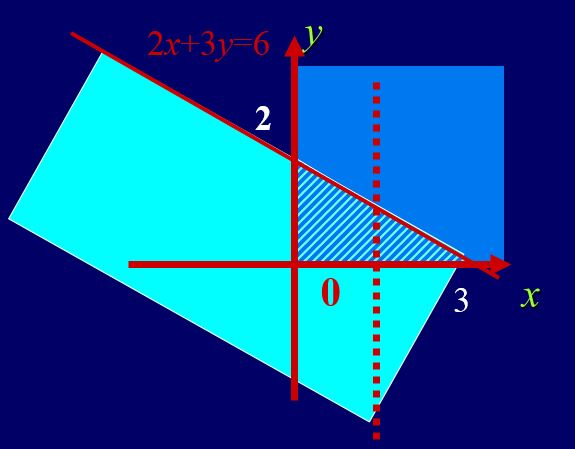
\includegraphics[width=5cm]{exam2.jpg}
  \end{figure}
\end{frame}

\subsection{边缘分布}
\begin{frame}
  \frametitle{边缘分布:随机向量的分量各自的概率分布}
  \begin{defi}[边缘分布] 在 $(X,Y)$ 的联合分布函数中,令 $y\uparrow +\infty$ 可得
    \begin{eqnarray*}
      \lim_{y\rightarrow+\infty}F(x,y)&=&\pause \lim_{y\rightarrow+\infty}P(X\le x, Y\le y)\\ &=& \pause P(X\le x,Y\le +\infty)=F(x,+\infty)
      \\
      &=&\pause P(X\le x):=F_1(x).    \end{eqnarray*}
  称 $F_1 (x)$ 为 $X$ 的边缘分布. \pause 类似的,$Y$ 的边缘分布为
\begin{eqnarray*}
F_2(y)=P(Y\le y)=\lim_{x\rightarrow+\infty}F(x,y)=F(+\infty,y)
\end{eqnarray*}

\end{defi}

\pause 从边缘分布的定义可知,若 $(X,Y)$ 的联合分布为 $F (x,y)$, 则
\begin{eqnarray*}
X\sim F_1(x)=F(x,+\infty)\\
Y\sim F_2(y)=F(+\infty, y)
\end{eqnarray*}
\end{frame}

\begin{frame}
	\frametitle{边缘分布的离散情形}
	\begin{itemize}[<+-|alert@+>]
		\item 边缘一词源于离散型情形。在二维离散型概率分布 $\{p_{ij}\}$ 的列表中,将各行求和写在表的最右一列,再将各列求和写在表的最下一行.
		\item 若 $(X,Y)$ 的联合分布列为 $\{p_{ij}\}$, 则 \pause %\vspace{-0.6cm}
		\begin{eqnarray*}
			&&X\mbox{的分布列为:} P (X=x_i)=\pause \sum_{j} P (X=x_i,Y=y_j)=\pause \sum_{j} p_{ij}=\pause p_{i\cdot};\\
			&& \pause Y\mbox{的分布列为:} P (Y=y_j)=\pause\sum_{i} P (X=x_i,Y=y_j)=\pause\sum_{i} p_{ij}=\pause p_{\cdot j}
		\end{eqnarray*}

	\end{itemize}
	\pause \vspace{-0.3cm}
	\begin{table}
		\centering
		\rowcolors[]{1}{blue!20}{blue!10}
		\begin{tabular}{|c|c|c|c|c|c|c|}
			\hline
			\rowcolor{blue!50}
			$i,j$ & 1  &2 &$\cdots$&$j$&$\cdots$ & $p_{i\cdot}$\\
			\hline
			1 & $p_{11}$ & $p_{12}$  & $\cdots$ &  $p_{1j}$& $\cdots$ & $p_{1\cdot}$\\
			2  & $p_{21}$ & $p_{22}$  &$\cdots$ &  $p_{2j}$  &$\cdots$ & $p_{2\cdot}$\\
			$\vdots$ & $\vdots$ & $\vdots$  &$\vdots$ &  $\vdots$ &$\vdots$& \\
			$i$ & $p_{i1}$ & $p_{i2}$  & $\cdots$ & $p_{ij}$ &$\cdots$ & $p_{i\cdot}$\\
			$\vdots$ & $\vdots$ & $\vdots$  &$\vdots$ &  $\vdots$ &$\vdots$& \\
			$p_{\cdot j}$& $p_{\cdot 1}$& $p_{\cdot 2}$& $\cdots$& $p_{\cdot j}$&$\cdots$& \\  \hline
		\end{tabular}
		% \caption{二维离散型分布列}
	\end{table}

\end{frame}
\begin{frame}
	\frametitle{边缘分布的连续情形}
	\begin{itemize}[<+-|alert@+>]
		\item 注意到
		\vspace{-0.4cm}\begin{eqnarray*}
			\hspace{-0.3cm}F_1(x)&=&P(X\le x)=\pause F(x,+\infty)=\pause \int_{-\infty}^x\int_{-\infty}^{+\infty}p(u,v)dudv\\
			&=&\pause \int_{-\infty}^x\underbrace{\left[\int_{-\infty}^{+\infty}p(u,v)dv\right]}_{p_1(u)}du=\pause \int_{-\infty}^xp_1(u)du
		\end{eqnarray*}
		\vspace{-0.4cm}   \pause  类似的有,\begin{eqnarray*}
			\hspace{-0.3cm}F_2(y)&=&P(Y\le y)=\pause F(+\infty,y)=\pause \int_{-\infty}^y\int_{-\infty}^{+\infty}p(u,v)dudv\\
			&=&\pause \int_{-\infty}^x\underbrace{\left[\int_{-\infty}^{+\infty}p(u,v)du\right]}_{p_2(v)}dv=\pause \int_{-\infty}^yp_2(v)dv
		\end{eqnarray*}
\item 对于连续型随机向量,其分量仍为连续型,相应的边缘密度分别为 $$p_1 (x)=\int_{-\infty}^{+\infty} p (x,y) dy,\quad  p_2 (y)=\int_{-\infty}^{+\infty} p (x,y) dx$$
\end{itemize}
\end{frame}
\subsection{常见的多维分布}
\begin{frame}
\frametitle{常见的多维离散型分布:多项分布}
\begin{itemize}[<+-|alert@+>]
\item 多项分布:进行 $n$ 次独立重复试验,每次试验有 $r$ 个互不相容的结果:$A_1,\cdots, A_r$ 之一发生;
\item 每次试验中 $A_i$ 发生的概率为 $p_i=P (A_i), i=1,\cdots,  r$ 且 $p_1+\cdots +p_r=1$;
\item 记 $X_i$ 为 $n$ 次独立试验中 $A_i$ 出现的次数,则 $(X_1,X_2,\cdots,X_r)$ 取值 $(n_1,n_2,\cdots,n_r)$ 的概率,即 $A_i,i=1,\cdots, r$ 出现 $n_i$ 次的概率为
\pause  \begin{eqnarray*}
	P(X_1=n_1,\cdots, X_r=n_r)=\dfrac{n!}{n_1!n_2!\cdots n_r!}p_1^{n_1}p_2^{n_2}\cdots p_r^{n_r}
\end{eqnarray*}
其中 $n=n_1+\cdots+n_r$;
\item 这个联合分布列称为 $r$ 项分布,又称多项分布,记作 $M (n,p_1,\cdots,p_r)$.
\item 上述概率是多项式 $(p_1+p_2+\cdots+p_r)^n$ 的一项,故其和为 1.
\item $r=2$ 时即为二项分布.
\end{itemize}
\end{frame}
\begin{frame}
	\frametitle{常见的多维离散型分布:多维超几何分布}
	\begin{itemize}
		\item 多维超几何分布:袋中有 $N$ 个球,其中有 $N_i$ 个 $i$ 号球,$i=1,2,\cdots, r$, 且 $N_1+N_2+\cdots +N_r=N$;
		\item 从中任取 $n$ 个球,若记 $X_i$ 为取出的 $n$ 个球中 $i$ 号球的个数,$i=1,2,\cdots, r$, 则 \pause
		\begin{eqnarray*}
			P(X_1=n_1,X_2=n_2,\cdots, X_r=n_r)=\dfrac{C_{N_1}^{n_1}C_{N_2}^{n_2}\cdots C_{N_r}^{n_r}}{C_{N}^n}
		\end{eqnarray*}
		其中 $n_1+n_2+\cdots+n_r=n$;
		\item $r=2$ 时即为超几何分布.\end{itemize}
\end{frame}
\begin{frame}
	\frametitle{多维均匀分布}
	\begin{defi}
		设 $D$ 为 $\mathbb{R}^ n$ 中的一个有界区域,其度量为 $S_D$, 如果多维随机变量 $(X_1,\cdots, X_n)$ 的联合密度函数为
		\begin{eqnarray*}
			p(x_1,\cdots,x_n)=\left\{
			\begin{array}{ll}
				\dfrac{1}{S_D}, &(x_1,x_2,\cdots,x_n)\in D\\
				0,&\mbox{其他}
			\end{array}\right.
		\end{eqnarray*}
		则称 $(X_1,\cdots,X_n)$ 服从 $D$ 上的多维均匀分布,记作 $(X_1,\cdots, X_n)\sim U (D)$.
	\end{defi}
	\vspace{0.5cm}

	\pause 二维均匀分布所描述的随机现象就是向平面区域 $D$ 中随机投点,如果该点的坐标 $(X,Y)$ 落在 $D$ 的子区域 $G$ 中的概率只与 $G$ 的面积有关,而与 $G$ 的位置无关,\pause 则
	\begin{eqnarray*}
		P((X,Y)\in G)=\iint_{G}p(x,y)dxdy=\iint_{G}\dfrac{1}{S_D}dxdy=\dfrac{S_G}{S_D}
	\end{eqnarray*}

\end{frame}
\begin{frame}
	\vspace{0.4cm}
	\begin{exam}
		设 $(X,Y)$ 服从单位圆 $D=\{(x,y):x^2+y^2<1\}$ 上的均匀分布,试求其边缘密度函数 (\textcolor{red}{非均匀分布}).
	\end{exam}
	\begin{columns}
		\pause   \column{3cm}
		% \vspace{-2cm}
		\begin{figure}[h]
			\centering
			\hspace{-1cm} 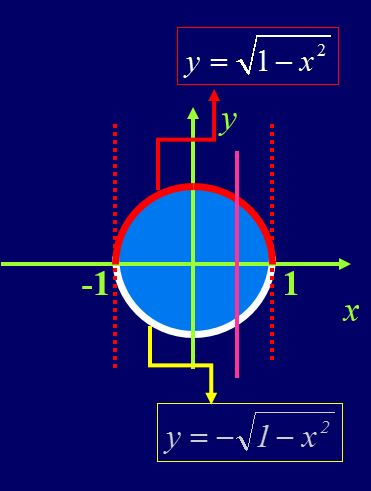
\includegraphics[width=4cm]{exam3.jpg}
		\end{figure}
		\pause %\vspace{0.7cm}
		\column{6.5cm}
		\pause $(X,Y)$ 的联合密度为
		\begin{eqnarray*}
			p(x,y)=\left\{
			\begin{array}{ll}
				\dfrac{1}{\pi}, & x^2+y^2<1\\
				0, & \mbox{其他}
			\end{array}\right.
		\end{eqnarray*}
		\pause 故当 $|x|\ge 1$, $p (x,y)=0$, 从而 $p_1 (x)=0$; 当 $|x|<1$ 时,
		\begin{eqnarray*}
			p_1(x)&=&\pause \int_{-\infty}^{+\infty}p(x,y)dy=\pause \int_{-\sqrt{1-x^2}}^{\sqrt{1-x^2}}\dfrac{1}{\pi}dy
			\\
			&=&\pause \dfrac{2}{\pi}\sqrt{1-x^2}
		\end{eqnarray*}\pause
		类似可得 $Y$ 的密度为 $p_2 (y)=\dfrac{2}{\pi}\sqrt{1-y^2}
		$
	\end{columns}
\end{frame}
\begin{frame}
	\frametitle{二维正态分布}
	\begin{defi}
		设参数 $\mu_1,\mu_2,\sigma_1,\sigma_2, \rho$ 满足 $\sigma_1>0,\sigma_2>0$ 及 $-1<\rho<1$, 称以
		\begin{eqnarray*}
			p(x,y)&=&\dfrac{1}{2\pi \sigma_1\sigma_2\sqrt{1-\rho^2}}\times\\
			&&\hspace{-1cm}\exp\bigg\{-\dfrac{1}{2(1-\rho^2)}\bigg[\dfrac{(x-\mu_1)^2}{\sigma_1^2}-\dfrac{2\rho(x-\mu_1)(y-\mu_2)}{\sigma_1\sigma_2}+\dfrac{(y-\mu_2)^2}{\sigma_2^2}\bigg]\bigg\}
		\end{eqnarray*}
		为密度函数的连续型分布为二维正态分布,记作 $$(X,Y)\sim N (\mu_1,\mu_2,\sigma_1^2,\sigma_2^2,\rho).$$
	\end{defi}

	\pause 后面我们会给出
	\begin{eqnarray*}
		\int_{-\infty}^{+\infty}  \int_{-\infty}^{+\infty}p(x,y)dxdy=1
	\end{eqnarray*}
	的证明.
\end{frame}

\begin{frame}
	\frametitle{二维正态分布密度图像}
	\vspace{0.2cm}
	\begin{figure}[h]
		\centering
		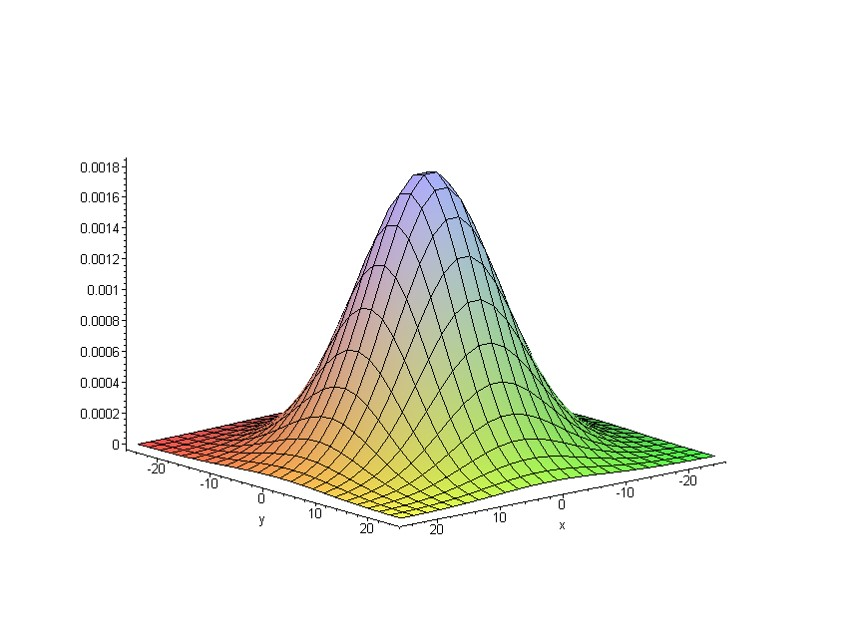
\includegraphics[width=11cm]{n2.jpg}
	\end{figure}
\end{frame}
\begin{frame}
	\frametitle{二维正态分布的边缘分布}
	\vspace{-0.3cm}
	\begin{thm}
		若 $(X,Y)$ 为二维正态分布 $N (\mu_1,\mu_2,\sigma_1^2,\sigma_2^2,\rho)$, 则 $$X\sim N (\mu_1,\sigma_1^2), \quad Y\sim N (\mu_2,\sigma_2^2)$$
	\end{thm}
	\vspace{-0.1cm}
	\pause\zheng $X$ 的边缘分布密度为
	{\small \begin{eqnarray*}
			p_1(x)&=&\pause \int_{-\infty}^{+\infty}\dfrac{1}{2\pi \sigma_1\sigma_2\sqrt{1-\rho^2}}\\
			&&\hspace{-0.3cm}\pause\cdot \exp\bigg\{-\dfrac{1}{2(1-\rho^2)}\bigg[\dfrac{(x-\mu_1)^2}{\sigma_1^2}-\dfrac{2\rho(x-\mu_1)(y-\mu_2)}{\sigma_1\sigma_2}+\dfrac{(y-\mu_2)^2}{\sigma_2^2}\bigg]\bigg\}dy\\
			&=&\pause \int_{-\infty}^{+\infty}\dfrac{1}{2\pi \sigma_1\sqrt{1-\rho^2}}\exp\left\{-\dfrac{u^2-2\rho uv+v^2}{2(1-\rho^2)}\right\}dv\\
			&=&\pause \int_{-\infty}^{+\infty}\dfrac{1}{2\pi \sigma_1\sqrt{1-\rho^2}}\exp\left\{-\dfrac{1}{2}\left[\left(\dfrac{v-\rho u}{\sqrt{1-\rho^2}}\right)^2+u^2\right]\right\}dv\\
			&=&\pause \dfrac{1}{\sqrt{2\pi}\sigma_1}e^{-\dfrac{(x-\mu_1)^2}{2\sigma_1^2}}\int_{-\infty}^{+\infty}\dfrac{1}{\sqrt{2\pi}} e^{-\dfrac{t^2}{2}}dt=\pause \dfrac{1}{\sqrt{2\pi}\sigma_1}e^{-\dfrac{(x-\mu_1)^2}{2\sigma_1^2}}
	\end{eqnarray*}}
	\pause 类似的可得 $Y\sim N (\mu_2,\sigma_2^2)$.
\end{frame}
%  \begin{frame}
	% \frametitle{作业}
	% P86-87. 习题 2.5.5: 3, 6, 7, 8, 9.
	%\end{frame}








\title[概率论]{第十二讲:条件分布与随机变量的独立性}
%\author[张鑫 {\rm Email: x.zhang.seu@foxmail.com} ]{\large 张 鑫}
\institute[东南大学数学学院]{\large \textrm{Email: xzhangseu@seu.edu.cn} \\ \quad  \\
	\large 东南大学 \quad 数学学院 \\
	\vspace{0.3cm}
%	\trc{公共邮箱: \textrm{zy.prob@qq.com}\\
	%	\hspace{-1.7cm}  密 \qquad 码: \textrm{seu!prob}}
}
\date{}





{ \setbeamertemplate{footline}{}
	\begin{frame}
		\titlepage
	\end{frame}
}
%\section{随机变量}
\subsection{条件分布}
\begin{frame}
	\frametitle{条件分布}
	\begin{itemize}[<+-|alert@+>]
		\item $(\Omega,\mathcal{F},P)$ 为一概率空间,任意固定 $B\in\mathcal{F}$ 且 $P (B)>0$, $P (\cdot|B)$ 仍为 $(\Omega,\mathcal{F})$ 上的概率;
		\item 对于 $(\Omega,\mathcal{F})$ 上的随机变量 $X$, 考虑其关于条件概率 $P (\cdot|B)$ 的分布即在概率空间 $(\Omega,\mathcal{F},P (\cdot|B))$ 上考虑 $X$ 的分布:
		\begin{eqnarray*}
			F(x|B):=P(X\le x|B)=\dfrac{P(X\le x, B)}{P(B)}, x\in R
		\end{eqnarray*}
		\item 现假定有另一随机变量 $Y$, 则当 $P (Y=y)>0$ 时,$F (x|Y=y)$ 则为已知 $Y=y$ 时 $X$ 的条件分布函数.
	\end{itemize}

\end{frame}

\begin{frame}
	\frametitle{离散型条件分布}
	\begin{defi}
		若离散型随机向量 $(X,Y)$ 的联合分布为 $\{p_{ij}\}$, 则当 $$P (Y=y_j)=p_{\cdot j}>0$$ 时,称
		\begin{eqnarray*}
			p_{i|j}:=P(X=x_i|Y=y_j)=\dfrac{p_{ij}}{p_{\cdot j}}, i=1,2,\cdots,
		\end{eqnarray*}
		为已知 $Y=y_j$ 时 $X$ 的条件分布. \pause 类似的,当 $P (X=x_i)=p_{i\cdot}>0$ 时,称
		\begin{eqnarray*}
			p_{j|i}:=P(Y=y_j|X=x_i)=\dfrac{p_{ij}}{p_{i\cdot}}
		\end{eqnarray*}
		为已知 $X=x_i$ 时 $Y$ 的条件分布.
	\end{defi}

\end{frame}
\begin{frame}
	\frametitle{离散型条件分布函数}
	根据上面的定义,给定 $Y=y_j$ 条件下 $X$ 的条件分布函数为
	\begin{eqnarray*}
		F(x|y_j)=\sum_{i:x_i\le x}P(X=x_i|Y=y_j)=\sum_{i:x_i\le x}p_{i|j}
	\end{eqnarray*}
	\pause 类似的给定 $X=x_i$ 条件下 $Y$ 的条件分布函数为
	\begin{eqnarray*}
		F(y|x_i)=\sum_{j:y_j\le y}P(Y=y_j|X=x_i)=\sum_{j:y_j\le y}p_{j|i}
	\end{eqnarray*}

\end{frame}
\begin{frame}
	\frametitle{连续型条件分布}
	\begin{itemize}[<+-|alert@+>]
		\item 设二维连续型随机变量 $(X,Y)$ 的联合密度函数为 $p (x,y)$, 边际密度函数分别为 $p_X (x), p_Y (y)$;
		\item 条件分布函数 $P (X\le x|Y=y)$: 因为 $P (Y=y)=0$, 故无法通过条件概率直接计算;
		\item $P(X\le x|Y=y):=\lim_{h\rightarrow 0}P(X\le x|Y\in[y,y+h])$;
		\item 根据如上定义:\vspace{-0.3cm}
		{\small \begin{eqnarray*}
				\hspace{-0.5cm} F(x|y)&:=&P(X\le x|Y=y)=\pause \lim_{h\rightarrow 0}\dfrac{P(X\le x, Y\in[y,y+h])}{P(Y\in[y,y+h])}\\
				&=&\pause \lim_{h\rightarrow 0}\dfrac{\int_{-\infty}^x\int_y^{y+h}p(u,v)dvdu}{\int_y^{y+h}p_Y(v)dv}
				=\pause \lim_{h\rightarrow 0}\dfrac{\int_{-\infty}^x\big\{\dfrac{1}{h}\int_y^{y+h}p(u,v)dv\big\}du}{\dfrac{1}{h}\int_y^{y+h}p_Y(v)dv}\\
				&&\hspace{-0.7cm}\pause \xlongequal[\mbox{积分中值定理}]{p (x,y),p_Y (y)\mbox{在} y\mbox{连续}}\pause \int_{-\infty}^x\dfrac{p (u,y)}{p_Y (y)} du\pause
		\end{eqnarray*}}%
		\item 这表明给定 $Y=y$ 时 $X$ 的条件分布仍为连续型,其密度函数为 $$p (x|y)=p (x,y)/p_Y (y).$$
	\end{itemize}
\end{frame}
\begin{frame}
	\frametitle{连续随机变量的条件分布函数及条件密度函数}
	\begin{defi}
		对一切使 $p_Y (y)>0$ 的 $y$, 给定 $Y=y$ 条件下 $X$ 的条件分布函数和条件密度函数分别为
		\begin{eqnarray*}
			F(x|y)&=&\int_{-\infty}^x\dfrac{p(u,y)}{p_Y(y)}du,\\
			p(x|y)&=&\dfrac{p(x,y)}{p_Y(y)}.
		\end{eqnarray*}
		同理,对一切使 $p_X (x)>0$ 的 $x$, 给定 $X=x$ 条件下 $X$ 的条件分布函数和条件密度函数分别为
		\begin{eqnarray*}
			F(y|x)&=&\int_{-\infty}^y\dfrac{p(x,v)}{p_X(x)}dv,\\
			p(y|x)&=&\dfrac{p(x,y)}{p_X(x)}.
		\end{eqnarray*}
	\end{defi}
\end{frame}
\begin{frame}
	\frametitle{连续场合的全概率公式和贝叶斯公式}
	\begin{itemize}[<+-|alert@+>]
		\item 由条件密度函数的定义可得
		\begin{eqnarray*}
			p(x,y)=p_X(x)p(y|x), \quad p(x,y)=p_Y(y)p(x|y)
		\end{eqnarray*}
		\item 对 $p (x,y)$ 求边际密度函数可得
		\begin{eqnarray*}
			p_X(x)&=&\pause \int_{-\infty}^{+\infty}p_Y(y)p(x|y)dy\pause \\
			\pause P(X\le x)&=&\pause \int_{-\infty}^x\bigg[\int_{-\infty}^{+\infty}p_Y(y)p(u|y)dy\bigg]du\\
			&=&\pause \int_{-\infty}^{+\infty}\bigg[\int_{-\infty}^xp(u|y)du\bigg]p_Y(y)dy\\
			&=&\pause \int_{-\infty}^{+\infty}P(X\le x|Y=y)dP(Y\le y)
			% p_Y(y)=\int_{-\infty}^{+\infty}p_X(x)p(y|x)dx, F(y)=\int_{-\infty}^{+\infty}\bigg[\int_{-\infty}^yp(v|x)dv\bigg]p_X(x)dx\\
		\end{eqnarray*}

	\end{itemize}
\end{frame}
\begin{frame}
	\frametitle{连续场合的全概率公式和贝叶斯公式}
	\begin{itemize}[<+-|alert@+>]
		\item 类似推导可得
		\begin{eqnarray*}
			p_Y(y)&=&\pause \int_{-\infty}^{+\infty}p_X(x)p(y|x)dx \\
			\pause P(Y\le y)&=& \pause \int_{-\infty}^{+\infty}P(Y\le y|X=x)dP(X\le x)
			% p_Y(y)=\int_{-\infty}^{+\infty}p_X(x)p(y|x)dx, F(y)=\int_{-\infty}^{+\infty}\bigg[\int_{-\infty}^yp(v|x)dv\bigg]p_X(x)dx\\
		\end{eqnarray*}
		\item 贝叶斯公式的密度函数形式:
		\begin{eqnarray*}
			p(x|y)=\dfrac{p(x,y)}{p_Y(y)}=\dfrac{p_X(x)p(y|x)}{\int_{-\infty}^{+\infty}p_X(x)p(y|x)dx}\\
			p(y|x)=\dfrac{p(x,y)}{p_X(x)}=\dfrac{p_Y(y)p(x|y)}{\int_{-\infty}^{+\infty}p_Y(y)p(x|y)dy}
		\end{eqnarray*}

	\end{itemize}
\end{frame}


\begin{frame}
	\begin{exam}
		若 $(X,Y)$ 为二维正态分布 $N (\mu_1,\mu_2,\sigma_1^2,\sigma_2^2,\rho)$, 试求给定 $Y=y$ 时 $X$ 的条件分布密度.\\
	\end{exam}


	\pause\jieda $X$ 的条件分布密度为
	\begin{eqnarray*}
		&&\hspace{-0.8cm}p(x|y)=\pause \dfrac{p(x,y)}{p_Y(y)}\\
		&=&\pause  \dfrac{\frac{1}{2\pi \sigma_1\sigma_2\sqrt{1-\rho^2}}\exp\big\{-\frac{1}{2(1-\rho^2)}\big[\frac{(x-\mu_1)^2}{\sigma_1^2}-\frac{2\rho(x-\mu_1)(y-\mu_2)}{\sigma_1\sigma_2}+\frac{(y-\mu_2)^2}{\sigma_2^2}\big]\big\}}{\frac{1}{\sqrt{2\pi}\sigma_2}\exp\big\{-\frac{(y-\mu_2)^2}{2\sigma_2^2}\big\}}\\
		&=&\pause \frac{\exp\big\{\frac{-1}{2\sigma_1^2(1-\rho^2)}\big[(x-\mu_1)^2-2\rho\frac{\sigma_1}{\sigma_2}(x-\mu_1)(y-\mu_2)+\rho^2\frac{\sigma_1^2}{\sigma_2^2}(y-\mu_2)^2\big]\big\}}{\sqrt{2\pi} \sigma_1\sqrt{1-\rho^2}}\\
		&=&\pause \frac{1}{\sqrt{2\pi} \sigma_1\sqrt{1-\rho^2}}\exp\big\{-\frac{1}{2\sigma_1^2(1-\rho^2)}\big[x-(\mu_1+\rho\frac{\sigma_1}{\sigma_2}(y-\mu_2)\big]^2\big\}\\
		&\sim&\pause  N(\mu_1+\rho\frac{\sigma_1}{\sigma_2}(y-\mu_2),\sigma_1^2(1-\rho^2)) \xlongequal{\rho=0} N(\mu_1,\sigma_1^2)
	\end{eqnarray*}
	\pause 类似可求得 $Y$ 关于 $X=x$ 的条件分布密度.
\end{frame}

\begin{frame}
	\begin{exam}
		设 $(X,Y)$ 服从单位圆 $D=\{(x,y):x^2+y^2<1\}$ 上的均匀分布,试求条件分布密度函数 $p (y|x)$.
	\end{exam}

	\jieda
	$(X,Y)$ 的联合密度及 $X$ 的边缘密度分别为
	\begin{eqnarray*}
		p(x,y)=\left\{
		\begin{array}{ll}
			\dfrac{1}{\pi}, & x^2+y^2<1,\\
			0, & \mbox{其他}
		\end{array}\right. ,\quad
		p_X(x)=\left\{\begin{array}{ll}
			\dfrac{2}{\pi}\sqrt{1-x^2}, & |x|<1,\\
			0, & \mbox{其他}.
		\end{array}\right.
	\end{eqnarray*}
	\pause 故
	\begin{eqnarray*}
		p(y|x)=\dfrac{p(x,y)}{p_X(x)}=\left\{
		\begin{array}{ll}
			\dfrac{1}{2\sqrt{1-x^2}}, & |y|\le \sqrt{1-x^2}\\
			0, &\mbox{其他}
		\end{array}
		\right.
	\end{eqnarray*}

\end{frame}


\subsection{随机变量的独立性}

\begin{frame}
	\frametitle{随机变量的独立性}
	\begin{itemize}[<+-|alert@+>]
		\item 首先我们回顾一下事件的独立性: $$P (AB)=P (A) P (B)\Leftrightarrow P (A|B)=P (A), \mbox{当} P (B)>0;$$
		\item 二维离散型随机变量
		\begin{eqnarray*}
			p_{i|j}:=\textcolor{red}{\dfrac{p_{ij}}{p_{\cdot j}}}=P (X=x_i|Y=y_j)\pause\xlongequal[\mbox{不影响概率}]{\mbox{若条件事件}} P (X=x_i)\textcolor{red}{=p_{i\cdot}};
		\end{eqnarray*}
		\item 故如果对任意的事件 $\{X=x_i\}, \{Y=y_j\}, i,j=1,2,\cdots,$ 均独立,我们则可称随机变量 $X,Y$ 独立,即 $X,Y$ 独立等价于
		\begin{eqnarray*}
			p_{ij}=p_{i\cdot}p_{\cdot j}, \quad i,j=1,2,\cdots,
		\end{eqnarray*}
		\item 此时的联合分布函数 $F (x,y)$ 为
		\begin{eqnarray*}
			\textcolor{red}{F(x,y)}&=&\pause P(X\le x,Y\le y)=\pause \sum_{x_i\le x}\sum_{y_j\le y}p_{ij}=\pause \sum_{x_i\le x}p_{i\cdot}\sum_{y_j\le y}p_{\cdot j}\\
			&=&\pause \sum_{x_i\le x}P(X=x_i)\sum_{y_j\le y}P(Y=y_j)=\pause \textcolor{red}{F_X(x)F_Y(y)}
		\end{eqnarray*}
	\end{itemize}
\end{frame}
\begin{frame}
	\frametitle{随机变量的独立性}
	\begin{itemize}[<+-|alert@+>]
		\item 二维连续型随机变量
		\begin{eqnarray*}
			F (x|y)&=&\int_{-\infty}^x\dfrac{p (u,y)}{p_Y (y)} du=P (X\le x|Y=y)\xlongequal[\mbox{不影响概率}]{\mbox{若条件事件}} P (X\le x)\\
			&=&\int_{-\infty}^xp_X(u)du\\
			&\Rightarrow& p(x,y)=p_X(x)p_Y(y)
		\end{eqnarray*}
		\item 此时,其分布函数
		\begin{eqnarray*}
			\textcolor{red}{F(x,y)}&=&P(X\le x, Y\le y)=\int_{-\infty}^x\int_{-\infty}^yp(u,v)dudv\\
			&=&\int_{-\infty}^xp_X(u)du\int_{-\infty}^yp_Y(v)dv=\textcolor{red}{F_X(x)F_Y(y)}
		\end{eqnarray*}
	\end{itemize}
\end{frame}
\begin{frame}
	\frametitle{随机变量独立性的定义}
	\begin{defi}
	 设 $n$ 维随机变量 $(X_1,X_2,\cdots,X_n)$ 的联合分布函数为 $F (x_1,
		\cdots,x_n)$, $F_i (x_i)$ 为 $X_i$ 的边缘分布函数。如果对任意的 $n$ 个实数 $x_1,x_2,\cdots, x_n$, 有
		\begin{eqnarray*}
			F(x_1,x_2,\cdots, x_n)=F_1(x_1)F_2(x_2)\cdots F_n(x_n)
		\end{eqnarray*}
		则称 $X_1,X_2,\cdots, X_n$ 相互独立。特别的,
	\end{defi}
	\pause
	\begin{enumerate}[<+-|alert@+>]
		\item 在离散随机变量场合,如果对任意 $n$ 个取值 $x_1,x_2,\cdots, x_n$, 有
		{\small     \begin{eqnarray*}
				P(X_1=x_1,X_2=x_2,\cdots,X_n=x_n)=P(X_1=x_1)P(X_2=x_2)\cdots P(X_n=x_n),
		\end{eqnarray*}}
		则称 $X_1,X_2,\cdots, X_n$ 相互独立.


		\item 在连续随机变量场合,如果对任意的 $n$ 个取值 $x_1,x_2,\cdots, x_n$, 有
		\begin{eqnarray*}
			p(x_1,x_2,\cdots, x_n)=p_1(x_1)p_2(x_2)\cdots p_n(x_n)
		\end{eqnarray*}
		则称 $X_1,X_2,\cdots, X_n$ 相互独立.
	\end{enumerate}
\end{frame}



 \title[概率论]{第十三讲:随机变量函数的分布}
% \author[张鑫 {\rm Email: x.zhang.seu@foxmail.com} ]{\large 张 鑫}
 \institute[东南大学数学学院]{\large \textrm{Email: xzhangseu@seu.edu.cn} \\ \quad  \\
 	\large 东南大学 \quad 数学学院 \\
 	\vspace{0.3cm}
 %	\trc{公共邮箱: \textrm{zy.prob@qq.com}\\
 	%	\hspace{-1.7cm}  密 \qquad 码: \textrm{seu!prob}}
 }
 \date{}



 	{ \setbeamertemplate{footline}{}
 		\begin{frame}
 			\titlepage
 		\end{frame}
 	}














% \section{随机变量}

 \subsection{随机变量函数的分布}
 \begin{frame}
 	\frametitle{一维离散型随机变量函数的分布}
 	\begin{thm}
 		设 $X\sim \{p_k\}$ 为一维离散型随机变量,若 $Z=f (X)$, 则对随机变量 $Z$ 的所有可能值 $z_k$ 有
 		\begin{eqnarray*}
 			P(Z=z_k)=\sum_{i:f(x_i)=z_k}p_i
 		\end{eqnarray*}
 	\end{thm}%
 	\pause%
 	\noindent\zheng 注意到 \vspace{-1cm}
 	\begin{eqnarray*}
 		\hspace{1.5cm} \{Z=z_k\}=\{f(X)=z_k\}=\cup_{i:f(x_i)=z_k}\{X=x_i\}
 	\end{eqnarray*}
 	\pause 故 $P (Z=z_k)=\sum_{i:f (x_i)=z_k} P (X=x_i)=\sum_{i:f (x_i)=z_k} p_i$.
 	\begin{exam}
 		若 $P (X=1)=P (X=-1)=0.25, P (X=0)=0.5$, 求 $Z=X^2$ 的分布.
 	\end{exam}

 	\jieda \pause$P(Z=1)=\sum_{i:x_i^2=1}p_i=P(X=1)+P(X=-1)=0.5$\\
 	\pause $$P(Z=0)=P(X=0)=0.5$$
 \end{frame}

 \begin{frame}
 	\frametitle{$Y=f (X): f (x)$ 严格单调且 $X$ 为连续型随机变量}
 	\begin{thm}
 		设 $X$ 是连续随机变量,其密度函数为 $p_X (x)$. $Y=f (X)$ 是另一个随机变量。若 $y=f (x)$ 严格单调,其反函数 $h (y)$ 有连续导数,则 $Y=f (X)$ 的密度函数为
 		\begin{eqnarray*}
 			p_Y(y)=\left\{
 			\begin{array}{ll}
 				p_X(h(y))|h'(y)|,& a\leq y\leq b\\
 				0,&\mbox{其他}
 			\end{array}
 			\right.
 		\end{eqnarray*}
 		其中 $a=\min\{f (-\infty), f (+\infty)\}, b=\max\{f (-\infty), f (+\infty)\}$.
 	\end{thm}

 	\pause \zheng 由 $f (x)$ 为严格单调函数可知:%
 	\begin{eqnarray*}
 		\hspace{-0cm} F_Y(y)&=&\pause P(Y\le y)=P(f(X)\le y)\\
 		&=&\pause \left\{
 		\begin{array}{ll}
 			\pause 0, & y<a\\
 			\pause 1, & y>b\\
 			\pause P (X\le h (y))=\pause \int_{-\infty}^{h (y)} p_X (x) dx, & a\leq y \leq b \mbox{且} f (x)\mbox{严格递增}\\
 			\pause P (X\ge h (y))=\pause \int_{h (y)}^{+\infty} p_X (x) dx, &a\leq y \leq b\mbox{且} f (x)\mbox{严格递减}
 		\end{array}
 		\right.
 	\end{eqnarray*}

 \end{frame}

 % \begin{frame}
 	%   从而 $Y$ 的密度函数为
 	%   \begin{eqnarray*}
 		%       p_Y(y)=\left\{
 		%       \begin{array}{ll}
 			%       p_X(h(y))|h'(y)|,& a<y<b\\
 			%       0,&\mbox{其他}
 			%     \end{array}
 		%                   \right.
 		%     \end{eqnarray*}

 	%                   \end{frame}
 \begin{frame}
 	\frametitle{几个常见的函数形式 $f$}
 	\begin{itemize}[<+-|alert@+>]
 		\item $f (x)=ax+b$ : 当 $X$ 为均匀分布,正态分布,伽玛分布时,求 $Y=f (X)$ 的分布密度;
 		\item 当 $X\sim N (\mu,\sigma^2)$ 时,可以验证 $aX+b\sim N (a\mu+b, a^2\sigma^2)$;
 		\item $f (x)=e^x$ : 当 $X$ 为均匀分布,正态分布,伽玛分布时,\\ 求 $Y=f (X)$ 的分布密度;
 		\item 对无单调性的函数 $f (x)$, 我们一般根据 $X$ 的分布密度想法求出 $Y$ 的分布函数 $F_Y (y)$,
 		\begin{eqnarray*}
 			F_Y(y)&=&P(Y\le y)=P(f(X)\le y)=P(X\in f^{-1}((-\infty, y]))\\
 			&=&\int_{f^{-1}((-\infty, y])}p_X(x)dx
 		\end{eqnarray*}
 		\item 然后对 $F_Y (y)$ 关于 $y$ 求导即可得到其分布密度 $p_Y (y)$.
 	\end{itemize}

 \end{frame}


% \begin{frame}
% 	\frametitle{两个问题}
% 	\begin{itemize}[<+-|alert@+>]
% 		\item 若 $X$ 为随机变量,对于怎样的 $f$ 才会有 $f (X)$ 仍然为随机变量?
% 		\item 给定分布函数 $F (x)$, 是否存在某个随机变量 $X$ 恰好使得其分布函数为给定的 $F (x)$?
% 	\end{itemize}
% \end{frame}
% \begin{frame}
% 	\frametitle{随机变量的 $p$ 分位数函数}
% 	\vspace{-0.3cm}
% 	\begin{defi}
% 		设 $X$ 是概率空间 $(\Omega,\mathcal{F},P)$ 上的随机变量,$F (x)$ 为其分布函数。对于 $p\in (0,1)$, 定义
% 		\begin{eqnarray*}
% 			F^{-1}(p):=\sup\{x:F(x)<p\}\pause =\inf\{x: F(x)\geq p\}.
% 		\end{eqnarray*}
% 		称 $F^{-1}(p)$ 为 $F$ 或 $X$ 的 $p$ 分位数,通常用 $x_p$ 或 $\xi_p$ 来表示.
% 	\end{defi}
%
%
% \end{frame}
%
% \begin{frame}
% 	\frametitle{随机变量的 $p$ 分位数函数的性质}
%
% 	\begin{itemize}[<+-|alert@+>]
% 		\item $F^{-1}(p)$ 关于 $p$ 单调不减:集合 $\{x:F (x)<p\}$ 关于 $p$ 单调不减,故其上确界也关于 $p$ 单调不减;
% 		\item 若 $x<F^{-1}(p)$, 则 $F (x)<p$: $F^{-1}(p)$ 是使得 $F (x)<p$ 的 $x$ 中的上确界;
% 		\item 若 $F (x)<p$, 则 $x<F^{-1}(p)$:\pause 由分布函数的右连续性知,若 $F (x)<p$, 对于给定的 $\epsilon:=\dfrac{p-F (x)}{2}$, 则必定存在充分小的 $\delta$, 使得
% 		\begin{eqnarray*}
% 			F(x+\delta)<F(x)+\epsilon=\dfrac{p+F(x)}{2}<p
% 		\end{eqnarray*}
% 		从而 $x<F^{-1}(p)$;\pause
% 		\item $x<F^{-1}(p)\Leftrightarrow F (x)<p$, 或等价的 $x\ge F^{-1}(p)\Leftrightarrow F (x)\ge p$;
% 		\item $P(X\le F^{-1}(p))=F(F^{-1}(p))\ge p$;
% 		\item $P(X\ge F^{-1}(p))=1-P(X<F^{-1}(p))$\\ \pause $=1-\lim_{\epsilon\rightarrow 0}P(X\le F^{-1}(p)-\epsilon)\pause \ge 1-p$
% 	\end{itemize}
%
% \end{frame}
%
%
% \begin{frame}
% 	\frametitle{$p$ 分位数函数的应用:随机变量的存在性}
% 	由前面所学知识易知:给定一个随机变量,我们可定义其分布函数,并且分布函数具有性质:单调不减,右连续,$F (-\infty)=0$, $F (+\infty)=1$. 那么反过来呢?
% 	\pause \begin{prob}
% 		给定一个分布函数 $F (x)$, 即函数 $F (x)$ 具有分布函数的性质:单调不减,右连续,$F (-\infty)=0$, $F (+\infty)=1$, 是否一定存在一个概率空间 $(\Omega,\mathcal{F},P)$ 及其上的随机变量 $X$ 使得其分布函数恰为 $F (x)$?
% 	\end{prob}
% 	\pause  \begin{thm}
% 		若 $F (x)$ 是右连续的单调不减函数,且 $F (-\infty)=0, F (+\infty)=1$, 则存在一个概率空间 $(\Omega,\mathcal{F},P)$ 及其上的随机变量 $X (\omega)$, 使 $X (\omega)$ 的分布函数恰好是 $F (x)$.
% 	\end{thm}
% \end{frame}
% \begin{frame}
% 	\frametitle{随机变量存在性的证明}
% 	\zheng
% 	\begin{itemize}[<+-|alert@+>]
% 		\item 取 $\Omega=[0,1]$, $\mathcal{F}$ 为 $[0,1]$ 上的 Borel 集全体,取 $P$ 为直线上的 Lebesgue 测度 (是长度概念的推广,但对一切 Borel 集有定义);
% 		\item 定义: $\theta (\omega)=\omega$, 则 $\theta (\omega)$ 是 $(\Omega,\mathcal{F},P)$ 上的随机变量,并且,对一切的 $0\le x\le 1$,
% 		\begin{eqnarray*}
% 			P(\theta(\omega)\le x)=P(\omega\in[0,x])=x;
% 		\end{eqnarray*}
% 		\item 考虑 $X (\omega):=F^{-1}(\theta (\omega))$, 则
% 		{\small\begin{eqnarray*}
% 				F_X(x)=P(X\le x)=\pause P(F^{-1}(\theta(\omega))\le x)\pause \xlongequal[p\le F(x)]{F^{-1}(p)\le x} P(\theta(\omega)\le F(x))=\pause F(x)
% 		\end{eqnarray*}}
%
%
% 	\end{itemize}
%
% \end{frame}
 \begin{frame}
 	\frametitle{多维随机变量函数的分布:离散情形}
 	\begin{thm}[离散卷积公式] 设 $X$ 与 $Y$ 为相互独立的非负整值随机变量,各有分布 $\{a_k\}$ 与 $\{b_k\}$. 则其和有分布
 		\begin{eqnarray*}
 			P(X+Y=n)=\sum_{k=0}^na_kb_{n-k}, n=0,1,2,\cdots.
 		\end{eqnarray*}
 	\end{thm}
 	\pause \zheng 注意到 $X$ 与 $Y$ 相互独立,故对任何的 $n=0,1,2,\cdots,$ 有
 	\begin{eqnarray*}
 		&&\hspace{-0.7cm}P(X+Y=n)=\pause \sum_{k=0}^\infty P(X+Y=n,X=k)=\pause \sum_{k=0}^n P(X+Y=n,X=k)\\
 		&=&\pause \sum_{k=0}^n P(X=k)P(X+Y=n|X=k)=\pause \sum_{k=0}^n P(X=k)P(Y=n-k|X=k)\\
 		&=&\pause \sum_{k=0}^n P(X=k)P(Y=n-k)=\sum_{k=0}^n a_kb_{n-k}
 	\end{eqnarray*}
 \end{frame}

 \begin{frame}
 	\frametitle{泊松分布的可加性}
 	\begin{exam}[泊松分布的可加性] 设随机变量 $X\sim P (\lambda_1), Y\sim P (\lambda_2)$, 且 $X,Y$ 相互独立,则 $Z=X+Y\sim P (\lambda_1+\lambda_2)$
 	\end{exam}

 	\pause \jieda 由题意知
 	\begin{eqnarray*}
 		P(Z=k)&=&\pause P(X+Y=k)=\pause \sum_{i=0}^\infty P(X=i, X+Y=k)\\
 		&=&\pause \sum_{i=0}^\infty P(X=i, Y=k-i)=\sum_{i=0}^kP(X=i,Y=k-i)\\
 		&=&\pause \sum_{i=0}^kP(X=i)P(Y=k-i)=\sum_{i=0}^n\bigg(\dfrac{\lambda_1^i}{i!}e^{-\lambda_1}\bigg)\bigg(\dfrac{\lambda_2^{k-i}}{(k-i)!}e^{-\lambda_2}\bigg)\\
 		&=&\pause \dfrac{e^{-(\lambda_1+\lambda_2)}}{\textcolor{red}{k!}}\sum_{i=0}^k\dfrac{\textcolor{red}{k!}}{i!(k-i)!}\lambda_1^i\lambda_2^{k-i}=\dfrac{(\lambda_1+\lambda_2)^k}{k!}e^{-(\lambda_1+\lambda_2)}\\
 		&&\pause k=0,1,\cdots,
 	\end{eqnarray*}

 \end{frame}

 \begin{frame}
 	\frametitle{泊松分布的可加性}

 	\begin{itemize}[<+-|alert@+>]
 		\item 泊松分布的上述性质可以叙述为:泊松分布的卷积仍是泊松分布,并记为
 		\begin{eqnarray*}
 			P(\lambda_1)*P(\lambda_2)=P(\lambda_1+\lambda_2);
 		\end{eqnarray*}
 		\item 这里的卷积是指 "寻求两具独立随机变量和的分布运算";
 		\item 上述泊松的性质可推广至有限个独立泊松随机变量之和的分布上去,即:
 		\begin{eqnarray*}
 			P(\lambda_1)*P(\lambda_2)*\cdots *P(\lambda_n)=P(\lambda_1+\lambda_2+\cdots+\lambda_n);
 		\end{eqnarray*}
 		\item 特别的,当 $\lambda_1=\lambda_2=\cdots=\lambda_n$ 时有
 		\begin{eqnarray*}
 			P(\lambda)*P(\lambda)*\cdots *P(\lambda)=P(n\lambda);
 		\end{eqnarray*}

 	\end{itemize}
 \end{frame}
 \begin{frame}
 	\frametitle{二项分布的可加性}
 	\begin{exam}[二项分布的可加性]
 		设随机变量 $X\sim B (n,p), Y\sim B (m,p)$, 且 $X,Y$ 独立,则 $X+Y\sim B (n+m,p)$. 特别的,若 $$X_i\sim B (1,p), i=1,2,\cdots, n, \mbox{则} X_1+X_2+\cdots+X_n\sim B (n,p).$$
 	\end{exam}
 \end{frame}

 \begin{frame}
 	\frametitle{多维随机变量函数的分布:连续情形的一般方法}
 	若 $Z=f (X_1,X_2,\cdots,X_n)$, $(X_1,X_2,\cdots,X_n)$ 的密度函数为 $p (x_1,x_2,\cdots,x_n)$, 则 $Y$ 的分布函数为
 	\begin{eqnarray*}
 		G(z)=P(Z\le z)=\int\cdots\int_{f(x_1,x_2,\cdots,x_n)\le z}p(x_1,x_2,\cdots,x_n)dx_1dx_2\cdots dx_n
 	\end{eqnarray*}

 \end{frame}
 \begin{frame}
 	\frametitle{二维随机变量和的分布 (卷积公式): $Z=X+Y$}
 	\begin{thm}
 		若 $Z=X+Y$, 而 $(X,Y)$ 的联合密度函数为 $p (x,y)$, 则
 		\begin{eqnarray*}
 			F(z)&=&P(Z\le z)=\pause \iint_{x+y\le z}p(x,y)dxdy\\
 			&=&\pause \int_{-\infty}^{+\infty}\int_{-\infty}^{z-x}p(x,y)dydx
 		\end{eqnarray*}
 		\pause 特别的,若 $X,Y$ 相互独立时有 $p (x,y)=p_1 (x) p_2 (y)$, 将其代入上式得 %\vspace{-0.6cm}
 		\pause \begin{eqnarray*}
 			F(z)&=&\pause \int_{-\infty}^{+\infty}dx\int_{-\infty}^{z-x}p_1(x)p_2(y)dy\\
 			&=& \pause  \int_{-\infty}^{+\infty}dx\int_{-\infty}^zp_1(x)p_2(u-x)du\\
 			&=& \pause  \int_{-\infty}^{z}\bigg[\int_{-\infty}^{+\infty}p_1(x)p_2(u-x)dx\bigg]du\\
 		\end{eqnarray*}
 		\pause 故其密度函数为 $p (z)=\int_{-\infty}^{+\infty} p_1 (z) p_2 (z-x) dx=\int_{-\infty}^{+\infty} p_1 (z-y) p_2 (y) dy$
 	\end{thm}
 \end{frame}
 \begin{frame}
 	\frametitle{正态分布的可加性}
 	\begin{exam}
 		设随机变量 $X\sim N (\mu_1,\sigma_1^2), Y\sim N (\mu_2,\sigma_2^2)$, 且 $X,Y$ 独立,则 $X+Y\sim N (\mu_1+\mu_2,\sigma_1^2+\sigma_2^2)$.
 	\end{exam}

 	\pause \zheng 显然 $Z=X+Y$ 仍在 $(-\infty,+\infty)$ 上取值。据卷积公式可得
 	{\small\begin{eqnarray*}
 			&&  \hspace{-2.4cm} p_z(z)=\int_{-\infty}^{+\infty}p_1(z-y)p_2(y)dy\\
 			&=&\dfrac{1}{2\pi\sigma_1\sigma_2}\int_{-\infty}^{+\infty}\exp\left\{-\dfrac{1}{2}\bigg[\dfrac{(z-y-\mu_1)^2}{\sigma_1^2}+\dfrac{(y-\mu_2)^2}{\sigma_2^2}\bigg]\right\}dy\\
 			&\xlongequal[B=\frac{(z-\mu_1)}{\sigma_1^2}+\frac{\mu_2}{\sigma_2^2}]{A=\frac{1}{\sigma_1^2}+\frac{1}{\sigma_2^2}}&\dfrac{1}{2\pi\sigma_1\sigma_2}\int_{-\infty}^{+\infty}\exp\left\{-\dfrac{1}{2}\bigg[A(y-\dfrac{B}{A})^2+\dfrac{(z-\mu_1-\mu_2)^2}{\sigma_1^2+\sigma_2^2}\bigg]\right\}dy\\
 			&=&\hspace{-0.5cm}\dfrac{\sqrt{2\pi}\sqrt{1/A}}{2\pi\sigma_1\sigma_2}e^{-\frac{(z-\mu_1-\mu_2)^2}{2(\sigma_1^2+\sigma_2^2}}\textcolor{red}{\int_{-\infty}^{+\infty}\frac{1}{\sqrt{2\pi}\sqrt{1/A}}\exp\big\{-\dfrac{(y-\dfrac{B}{A})^2}{2(\sqrt{1/A})^2}\big\}dy}\\
 			&=&\dfrac{1}{\sqrt{2\pi}\sigma_1\sigma_2\sqrt{A}}e^{-\frac{(z-\mu_1-\mu_2)^2}{2(\sigma_1^2+\sigma_2^2)}}=\dfrac{1}{\sqrt{2\pi}\sqrt{\sigma_1^2+\sigma_2^2}}e^{-\dfrac{(z-\mu_1-\mu_2)^2}{2(\sigma_1^2+\sigma_2^2)}}
 	\end{eqnarray*}}

 \end{frame}
 \begin{frame}
 	\frametitle{正态分布的可加性}
 	\begin{itemize}[<+-|alert@+>]
 		\item 若 $X\sim N (\mu,\sigma^2)$, 则对任意非零常数 $a$ 有,$aX\sim N (a\mu,a^2\sigma^2)$;
 		\item 若 $X_i\sim N (\mu_i,\sigma_i^2), i=1,2,\cdots, n$ 为 $n$ 个独立的正态随机变量,则其线性组合仍服从正态分布,即
 		\begin{eqnarray*}
 			a_1X_1+a_2X_2+\cdots+a_nX_n\sim N(\mu_0,\sigma_0^2)
 		\end{eqnarray*}
 		其中 $\mu_0=\sum_{i=1}^na_i\mu_i, \sigma_0^2=\sum_{i=1}^na_i^2\sigma_i^2$.


 	\end{itemize}
 \end{frame}

 \begin{frame}
 	\frametitle{Gamma 分布的可加性}
 	\begin{exam}
 		若 $X\sim \Gamma (\alpha_1,\lambda), Y\sim \Gamma (\alpha_2,\lambda)$, 且 $X,Y$ 独立,则 $$Z=X+Y\sim \Gamma (\alpha_1+\alpha_2,\lambda).$$
 	\end{exam}

 	\pause \begin{exam}
 		若 $X_i\sim \exp (\lambda)=\Gamma (1,\lambda), i=1,2,\cdots,n$, 且相互独立独立,则
 		\begin{eqnarray*}
 			X_1+X_2+\cdots+X_n\sim \Gamma(n,\lambda).
 		\end{eqnarray*}
 	\end{exam}

 	\pause
 	\begin{exam}
 		若 $X_i\sim \chi^2 (n_i)=\Gamma (\dfrac{n_i}{2},\dfrac{1}{2}), i=1,2,\cdots,m$, 且相互独立独立,则
 		\begin{eqnarray*}
 			X_1+X_2+\cdots+X_m&\sim& \Gamma(\dfrac{n_1+n_2+\cdots+n_m}{2},\dfrac{1}{2})\\
 			&=& \chi^2(n_1+n_2+\cdots+n_m)  \end{eqnarray*}

 	\end{exam}



 \end{frame}

 \begin{frame}
 	\frametitle{二维随机变量商的分布: $Z=X/Y$}
 	\vspace{-0.3cm}
 	\begin{thm}[商的密度] 如果随机变量 $(X,Y)$ 的联合密度函数为 $p (x,y)$, 则它们的商 $Z:=X/Y$ 仍为连续型,且其密度为
 		\begin{eqnarray*}
 			p(z)=\int_{-\infty}^{+\infty} |y|p(zy,y)dy.
 		\end{eqnarray*}
 	\end{thm}
 	\pause \zheng 商的分布函数为
 	\vspace{-0.3cm}
 	\begin{eqnarray*}
 		F(z)&=&\pause P(X/Y\le z)=\pause \iint_{x/y\le z}p(x,y)dxdy\\
 		&=&\pause \iint_{x/y\le z, y>0}p(x,y)dxdy+\iint_{x/y\le z,y<0}p(x,y)dxdy\\
 		&=&\pause \int_0^{+\infty} dy\int_{-\infty}^{yz}p(x,y)dx+\int_{-\infty}^0dy\int_{yz}^{+\infty}p(x,y)dx\\
 		&=&\pause \int_0^{+\infty} dy\int_{-\infty}^{z}yp(yu,y)du+\int_{-\infty}^0dy\int_{z}^{-\infty}yp(yu,y)du\\
 		&=&\pause \int_{-\infty}^{z}\bigg[\int_{-\infty}^{+\infty}|y|p(yu,y)dy\bigg]du
 	\end{eqnarray*}

 \end{frame}
 \begin{frame}
 	\frametitle{多维独立随机变量的最大 (小) 值分布}
 	\begin{thm}
 		若 $X_1,X_2,\cdots,X_n$ 是相互独立的随机变量,其各自的分布为 $F_k (x), k=1,2,
 		\cdots, n$, 若记
 		\begin{eqnarray*}
 			\overline{X}:=\max_{k=1}^nX_k, \quad \underline{X}=\min_{k=1}^nX_k
 		\end{eqnarray*}
 		则
 		\begin{eqnarray*}
 			P(\overline{X}\le x)=\Pi_{k=1}^nF_k(x),\quad  P(\underline{X}\le x)=1-\Pi_{k=1}^n(1-F_k(x))
 		\end{eqnarray*}
 	\end{thm}
 	\pause \zheng $\overline{X},\underline{X}$ 的分布函数为
 	\begin{eqnarray*}
 		F_{\overline{X}}(x)&=&P(\overline{X}\le x)=\pause P(X_1\le x,X_2\le x,\cdots, X_n\le x)\\
 		&=&\pause  \Pi_{k=1}^nP(X_k\le x)=\Pi_{k=1}^nF_k(x)\\
 		F_{\underline{X}}(x)&=& \pause 1-P(\underline{X}>x)=1-P(X_1>x,\cdots, X_n>x)\\
 		&=&\pause 1-\Pi_{k=1}^nP(X_k>x)=1-\Pi_{k=1}^n(1-F_k(x))
 	\end{eqnarray*}

 \end{frame}
 \begin{frame}
 	\frametitle{独立同分布情形下的最大最小值分布}
 	\begin{coro}
 		若上述定理中的 $F_k$ 均相同为 $F (x)$, 并且假设 $F (x)$ 具有分布密度 $p (x)$, 则 $\overline{X},\underline{X}$ 分布密度分别为
 		\begin{eqnarray*}
 			p_{\overline{X}}(x)&=&n[F(x)]^{n-1}p(x),\\
 			p_{\underline{X}}(x)&=&n[1-F(x)]^{n-1}p(x)
 		\end{eqnarray*}
 	\end{coro}

 	\pause

 	\textcolor{red}{思考}: 计算 $(\overline{X},\underline{X})$ 的联合分布函数.

 \end{frame}

 \begin{frame}
 	\frametitle{随机向量函数的联合分布:一般情形}
 	求连续型随机向量的函数的分布最一般的提法是:

 	设已知 $(X_1,X_2,\cdots,X_n)$ 的联合密度函数 $p (x_1,x_2,\cdots, x_n)$, 而
 	\begin{eqnarray}
 		\label{eq:yfx}
 		\left\{
 		\begin{array}{l}
 			Y_1=f_1(X_1,X_2,\cdots,X_n)\\
 			Y_2=f_2(X_1,X_2,\cdots,X_n)\\
 			\cdots\\
 			Y_m=f_m(X_1,X_2,\cdots,X_n)
 		\end{array}
 		\right.
 	\end{eqnarray}
 	求随机变量 $(Y_1,Y_2,\cdots,Y_n)$ 的分布.

 	\pause
 	\begin{itemize}[<+-|alert@+>]
 		\item 保证 $(Y_1,Y_2,\cdots, Y_n)$ 是随机向量:只需 $f_i, i=1,2,\cdots, m$ 是 Borel 函数即可;
 		\item 我们需要利用 $(X_1,\cdots, X_n)$ 的分布密度计算 $(Y_1,\cdots,Y_n)$, 故我们需要从 \eqref{eq:yfx} 中反解出 $(X_1,\cdots,X_n)$ 即要求方程组 \eqref{eq:yfx} 有解:
 		\begin{itemize}
 			\item 若 $m>n$, 既使对线性函数 $f_i$ 也不能保证方程组有解;
 			\item 若 $m<n$, 我们可以增补 $Y_j=X_j, j=m+1,\cdots, n$ 化为 $m=n$ 的情形;
 			\item 故我们只考虑 $m=n$ 的情形.
 		\end{itemize}

 	\end{itemize}

 \end{frame}
 \begin{frame}
 	\frametitle{随机向量函数的联合分布:一般情形}
 	\begin{thm}\hspace{-0.3cm}
 		设随机向量 $(X_1,X_2,\cdots,X_n)$ 的联合密度函数 $p (x_1,x_2,\cdots, x_n)$, 而 $Y_k=f_k (X_1,\cdots,X_n), k=1,2,\cdots,n$.
 		% \begin{eqnarray}
 			%   \label{eq:yfx2}
 			%   \left\{
 			%     \begin{array}{l}
 				%       Y_1=f_1(X_1,X_2,\cdots,X_n)\\
 				%       \cdots\\
 				%       Y_n=f_m(X_1,X_2,\cdots,X_n)
 				%     \end{array}
 			%   \right.
 			% \end{eqnarray}
 		若假设每个 $f_k$ 均为 $n$ 维 Borel 函数,并且对 $(Y_1,\cdots, Y_n)$ 的每一组可能值 $(y_1,\cdots,y_n)$, 方程组
 		\begin{eqnarray}\label{eq:yxf2}
 			\left\{
 			\begin{array}{l}
 				y_1=f_1(x_1,\cdots,x_n)\\
 				\cdots\\
 				y_n=f_n(x_1,\cdots,x_n)
 			\end{array}
 			\right.
 		\end{eqnarray}
 		有唯一解 \vspace{-0.7cm}\begin{eqnarray}\label{eq:yxf3}
 			\left\{\begin{array}{l}
 				x_1=h_1(y_1,\cdots,y_n)\\
 				\cdots\\
 				x_n=h_n(y_1,\cdots,y_n)
 			\end{array}
 			\right.
 		\end{eqnarray}
 		并且每个 $h_k (y_1,\cdots,y_n)$ 有连续的一阶偏导数。那么 $(Y_1,\cdots, Y_n)$ 是连续型随机向量,并且有联合密度函数
 		\begin{eqnarray*}
 			q(y_1,\cdots,y_n)=\left\{
 			\begin{array}{l}
 				p\big(h_1(y_1,\cdots,y_n),\cdots, h_n(y_1,\cdots,y_n)\big)|J|\\
 				0,  \mbox{若}(y_1,\cdots,y_n)\mbox{使}\eqref{eq:yxf2}\mbox{无解}
 			\end{array}
 			\right.
 		\end{eqnarray*}
 		其中 $J$ 为变换 \eqref{eq:yxf3} 的 Jacobi 行列式.
 	\end{thm}
 \end{frame}
 \begin{frame}
 	\frametitle{随机向量函数的联合分布:一般情形}

 	\zheng $(Y_1,\cdots,Y_n)$ 的联合分布函数为
 	\begin{eqnarray*}
 		&&\hspace{-0.7cm} F(u_1,\cdots,u_n)=\pause P(Y_1\le u_1,\cdots,Y_n\le u_n)\\
 		&=&\pause \int_{f_1(x_1,\cdots,x_n)\le u_1}\cdots\int_{f_n(x_1,\cdots,x_n)\le u_n}p(x_1,\cdots,x_n)dx_1\cdots dx_n\\
 		&=&\pause \int_{-\infty}^{u_1}\cdots\int_{-\infty}^{u_n}p\big(h_1(y_1,\cdots,y_n),\cdots, h_n(y_1,\cdots,y_n)\big)|J|dy_1\cdots dy_n\\
 	\end{eqnarray*}
 	\pause 故 $(Y_1,\cdots, Y_n)$ 是连续型随机向量,并且有联合密度函数
 	\begin{eqnarray*}
 		q(y_1,\cdots,y_n)=\left\{
 		\begin{array}{l}
 			p\big(h_1(y_1,\cdots,y_n),\cdots, h_n(y_1,\cdots,y_n)\big)|J|\\
 			\\
 			0,  \mbox{若}(y_1,\cdots,y_n)\mbox{使}\eqref{eq:yxf2}\mbox{无解}
 		\end{array}
 		\right.
 	\end{eqnarray*}

 	\pause \textcolor{red}{注:} 若 Jacobi 行列式 $J$ 不易计算时,可计算 $J^{-1}$ 即变换 \eqref{eq:yxf2} 的 Jacobi 行列式.
 \end{frame}

 \begin{frame}
 	\frametitle{随机变量积的分布}
 	\begin{exam}
 		设随机向量 $(X,Y)$ 的联合密度函数为 $p (x,y)$. 则 $U=XY$ 的密度函数为
 		\begin{eqnarray*}
 			p_U(u)=\int_{-\infty}^{+\infty}p(\frac{u}{v},v)\dfrac{1}{|v|}dv
 		\end{eqnarray*}
 	\end{exam}%
 	\pause \zheng 增补变量 $V=Y$, 则
 	$ \left\{
 	\begin{array}{l}
 		u=xy,\\
 		v=y,
 	\end{array}
 	\right.$
 	的反函数为 \pause $ \left\{
 	\begin{array}{l}
 		x=\dfrac{u}{v},\\
 		y=v,
 	\end{array}
 	\right.$. \pause 其 Jacobi 行列式为
 	\begin{eqnarray*}
 		J=\left|
 		\begin{array}{cc}
 			\dfrac{1}{v} & -\dfrac{u}{v^2}\\
 			& \\
 			0      & 1
 		\end{array}
 		\right|=\dfrac{1}{v},
 	\end{eqnarray*}
 	\pause 故 $(U,V)$ 的联合密度函数为 $q (u,v)=p (\dfrac{u}{v},v)\dfrac{1}{|v|}$. \pause 对 $q (u,v)$ 关于 $v$ 积分便可得 $U=XY$ 的密度函数. \pause (\textcolor{red}{随机变量商的密度也可类似求出})
 \end{frame}



